%\documentclass[serif, aspectratio=169]{beamer}  % for 16:9 ratio
\documentclass[serif]{beamer}  % for 4:3 ratio
\usepackage[T1]{fontenc} 
\usepackage{hyperref}
\usepackage{latexsym,amsmath,xcolor,multicol,booktabs,calligra}
\usepackage{graphicx,pstricks,listings,stackengine}
\usepackage{multimedia}

\author{
    Valeria De Stasio \\ 
    \and  
    Christian Faccio \\
    \and  
    Carlos Velázquez Fernández
}
\title{Detection and tracking of fishes: \\ an analysis of the YOLOv8 model}
\date{\small July 25, 2025}
\usepackage{UoWstyle}

% defs
\def\cmd#1{\texttt{\color{red}\footnotesize $\backslash$#1}}
\def\env#1{\texttt{\color{blue}\footnotesize #1}}
\definecolor{deepblue}{rgb}{0,0,0.5}
\definecolor{deepred}{RGB}{153,0,0}
\definecolor{deepgreen}{rgb}{0,0.5,0}
\definecolor{halfgray}{gray}{0.55}

\lstset{
    basicstyle=\ttfamily\tiny,
    keywordstyle=\bfseries\color{deepblue},
    emphstyle=\ttfamily\color{deepred},    % Custom highlighting style
    stringstyle=\color{deepgreen},
    numbers=left,
    numberstyle=\tiny\color{halfgray},
    rulesepcolor=\color{red!20!green!20!blue!20},
    frame=shadowbox,
}


\begin{document}

\begin{frame}
    \vfill
    \begin{center}
        
\includegraphics[keepaspectratio, scale=0.15]{images/logo.jpg}
        
        \vspace{1cm}
        
        \begin{beamercolorbox}[wd=\textwidth,center,rounded=true]{title}
            {\textbf{Detection, classification and tracking of fishes: \\ an analysis of the YOLOv8 model}}
        \end{beamercolorbox}
        
        \vspace{1cm}
        
        {July 25, 2025}
    \end{center}
    \vfill
\end{frame}

\begin{frame}    
\tableofcontents[sectionstyle=show,
subsectionstyle=show/shaded/hide,
subsubsectionstyle=show/shaded/hide]
\end{frame}

\section{Theory}

\begin{frame}
\frametitle{Fish detection problem}
\end{frame}

\begin{frame}
\frametitle{History of fish detection}
\end{frame}

\begin{frame}
\frametitle{YOLO}
\end{frame}

\begin{frame}
\frametitle{YOLOv8}
\end{frame}

\begin{frame}
\frametitle{Sub-things to explain}
\end{frame}

\section{Detection}

\begin{frame}
\frametitle{Datasets}
\end{frame}

\begin{frame}[fragile]
\frametitle{Configuration files}
\begin{columns}
\begin{column}{0.45\textwidth}
\begin{lstlisting}[language=python]
train: path_to_train/images
val: path_to_val/images
test: path_to_test/images

nc: 1
names: ['Fish']
\end{lstlisting}
\end{column}

\begin{column}{0.45\textwidth}
\begin{lstlisting}[language=python]
train: path_to_train/images
val: path_to_val/images
test: path_to_test/images

nc: 23
names: [
  'Caranx_sexfasciatus',
  'F1', 
  'F2',
  'F3', 
  'F4',
  'F5',
  'F6',
  'F7',
  'Acanthopagrus_palmaris',
  'Lutjanus_russellii',
  'acanthopagrus_and_caranx',
  'acanthopagrus_palmaris', 
  'Gerres',
  'Caranx',
  'Amniataba_caudivittatus',
  'gerres_2',
  'gerres',
  'Epinephelus',
  'Fish',
  'juvenile',
  'palmaris',
  'EJP',
  'caudivittatus'
]
\end{lstlisting}
\end{column}
\end{columns}
\end{frame}

%probably multiple frames for this

\begin{frame}
\frametitle{YOLOv8 models}
\end{frame}

\begin{frame}
\frametitle{Training}
\end{frame}

\begin{frame}
\frametitle{Inference}
\end{frame}

\section{Tracking}

\begin{frame}
    \frametitle{The Tracking Challenge: Occlusion \& ID Switches}
    
    \textbf{Problem:} In complex underwater scenes, fish are frequently occluded by objects or other fish.
    \vspace{1em}
            
    A naive tracker will often:
    \begin{itemize}
        \item \textbf{Lose the track} entirely when the fish disappears.
        \item \textbf{Create a new ID} when the fish reappears (\textcolor{deepred}{ID Switch}).
    \end{itemize}
    
    \vspace{1em}
    \textbf{Goal:} Maintain a persistent, correct ID for each fish despite occlusions.
\end{frame}


\begin{frame}
    \frametitle{The ByteTrack Algorithm}
    
    \begin{columns}[T]
        \begin{column}{0.5\textwidth}
            \textbf{Stage 1: High-Confidence Match}
            \begin{itemize}
                \item Uses motion prediction (Kalman Filter) to estimate the next position of existing tracks.
                \item Matches these predictions with high-confidence detections from the YOLO model.
            \end{itemize}
        \end{column}
        
        \begin{column}{0.5\textwidth}
            \textbf{Stage 2: Low-Confidence Match}
            \begin{itemize}
                \item Instead of discarding low-confidence detections, it keeps them.
                \item It attempts to match these "doubtful" detections to the tracks that were lost in Stage 1.
            \end{itemize}
        \end{column}
    \end{columns}
    
\end{frame}

\begin{frame}
    \frametitle{Occlusion Example}
    
    \begin{columns}[T,totalwidth=\textwidth] 
        \begin{column}{0.32\textwidth}
            \centering
            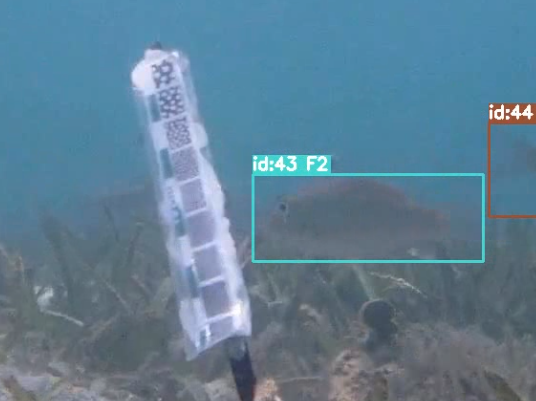
\includegraphics[width=\linewidth]{images/occlusion_1.png}
            \vspace{0.5em}
            \tiny
            \textbf{1. Before Occlusion} \\
            The fish ID 43 is clearly visible and being tracked.
        \end{column}
        
        \begin{column}{0.32\textwidth}
            \centering
            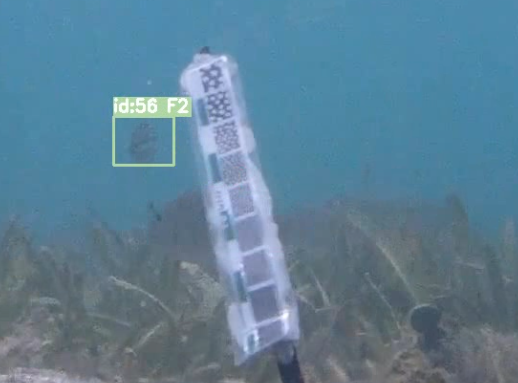
\includegraphics[width=\linewidth]{images/occlusion_2.png}
            \vspace{0.5em}
            \tiny
            \textbf{2. During Occlusion} \\
            Fish ID 43 is now hidden behind an object.
        \end{column}
        
        \begin{column}{0.32\textwidth}
            \centering
            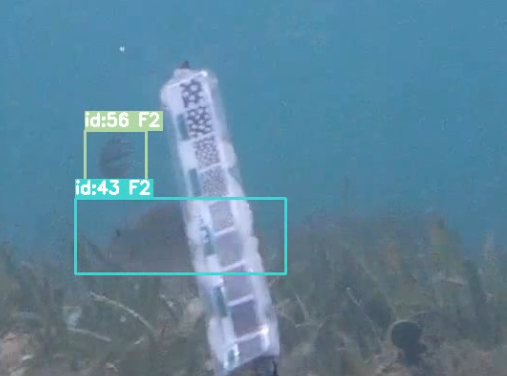
\includegraphics[width=\linewidth]{images/occlusion_3.png}
            \vspace{0.5em}
            \tiny
            \textbf{3. After Occlusion} \\
            The fish reappears. ByteTrack re-identifies it as ID 43.
        \end{column}
    \end{columns}
\end{frame}


\section{Results}

\section{Conclusions}

\end{document}
